As mentioned in the introduction, see chapter \ref{introduction}. The RRT-connect should comply some constraints. To illustrate those constraints more clearly and intuitively, a figure present in \ref{fig:humancenter} will illustrate it better.


\begin{figure}[htp]
  \centering
  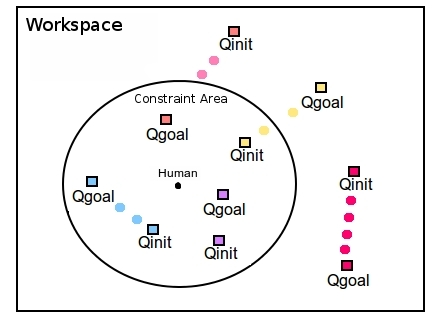
\includegraphics[width=0.5\textwidth]{images/humancenter.jpg}
  \caption{This figure shows the top of the workcell of the UR1 robot. The circle or cylinder is the constraint area, where the human center is at the center of the circle. Blue Qinit and Qgoal is allowed. Purple Qinit and Qgoal not allowed. Yellow Qinit and Qgoal allowed. Red Qinit and Qgoal allowed. Pink Qinit and Qgoal not allowed.} 
  \label{fig:humancenter}
\end{figure}

This figure illustrates five possibilities of ways of motion. It's assumed that the step size is reasoning small. 
Here we denote HC(X) to be the distance from X to human center.
\begin{itemize}
\item The red planning works completely because both configurations(Qs) are outside of the constraint area(CA), and if we except that the path between them is outside the CA all the time. 
	\begin{itemize}
	\item HC(all path points) > threshold. Threshold is the distance of the radius or safety length. 
	\end{itemize} 
\item The yellow planning is also accepted, if path inside the CA is increasing each step. 
	\begin{itemize}
	\item When path points are inside the CA it must not violate this condition, 
	that HC(path point) > HC(previous path point).
	\item When previous path point is outside of the CA, it must not violate the 
	HC(path point) > threshold.
	\end{itemize}
\item Purple planning is not allowed because the Qgoal is inside the CA and also closer to the human center than the Qinit.
\item Blue planning where both Qinit and Qgoal are inside the CA. It's only possible if each new step from Qinit increasing the distance to the human center. This means that the path never can get outside and inside again of the CA.
	\begin{itemize}
	\item  HC(path point) >  HC(previous path point).
	\item  HC(path point) <  HC(Qgoal).
	\end{itemize} 
\item Pink planning is not allowed because Qgoal is inside the CA and Qinit is not.
\end{itemize}

\section{Pseudo code of the constraint checking}
It should be assumed that constraints are tested in a straight forward approach. Meaning that the distance is a straight forward path between two point with a fixed step-size. Where distance is split into N, based on the step-size. Thus n = 1,2,3...N.

\subsection{Constraint checking of QINIT and QGOAL}
In the beginning Qinit and Qgoal have to validated to ensure that the path at all is possible based on constraints. The pseudo code for this action is present in listing \ref{listing:QinitQgoal}, its purpose is avoidance of purple and pink planning. The method parameters are HC(Qinit) and HC(Qgoal). If distance\_init is larger than distance\_goal and distance\_goal is inside the CA, which correspond to purple and pink planning. This will be discarded by returning false. If it returning true, that Qinit and Qgoal are valid and ready to be continue to check the path between them.

\begin{lstlisting}[caption=Peseudo code of validate function of Qinit and Qgoal, label=listing:QinitQgoal]
CheckQinitQgoal(distance_Qinit, distance_Qgoal)
	if(distance_Qinit > distance_Qgoal && distance_Qgoal < Threshold)
		return false;
	else 
		return true;
\end{lstlisting}

\subsection{Constraint checking of TINIT}
The actually constraint checking is present in listing \ref{listing:constraints}. Please note that the constraints are different depending on which tree it's acting on.
The input to the method is the distance = HC(Qi), HC(distance\_Qinit), HC(distance\_goal)  and HC(prevoius Qi). Qi is a point from the straight forward checking.
Please note, that first run previous Qi will be Qinit or Qgoal.
In line 2, where whichtree() is returning the name of the tree. 

The first possibility is when the tree is "TINIT". Here the planning will only be constraint of two conditions that should be avoided. If one of the conditions are true, then it will return false, that indicating the path to be constrained. False for none constraints.
\begin{itemize}
\item Distance is inside the CA and distance is less than the previous distance. Meaning that the path distance to hum,an center will not be increasing inside the CA. Here the blue and yellow planning will be doable.
\item Qgoal is inside CA and distance will be larger than distance\_Qgoal. This prevent the blue path to get outside the CA or larger than distance\_Qgoal.
\end{itemize}

\subsection{Constraint checking of TGOAL}
For the second case when the tree is "TGOAL", where three set of conditions are contributing a path to be constrained.
\begin{itemize}
\item Distance can't be less than distance\_Qinit, if Qinit is inside the CA. This prevent blue and yellow path to get closer to human center 
\item Qi can't be inside CA if Qinit is outside of CA. This prevent the red path to get inside CA.
\item Distance can't be larger than distance\_prevQi, if previous Qi is inside CA. This ensure that blue and yellow will have increasing path distance to human center inside the CA.
\end{itemize}

\begin{lstlisting}[caption=Peseudo code of constraint checking, label=listing:constraints]
CheckConstraint(distance, distance_Qinit, distance_Qgoal, distance_prevQi)
	if(whichTree() == TINIT)
		if(distance_Qgoal <= threshold && distance > distance_Qgoal)	
			b = false;
		else if(distance <= threshold && distance < distance_prevQi)
			b = false;
		else
			b = true;
	else if(whichTree() == TGOAL)
		if(distance < distance_Qinit && distance_Qinit <= threshold)
			b = false;
		else if(distance <= threshold && Qinit > threshold)	
			b = false;
		else if(distance_prevQi <= threshold && distance >= distance_prevQi)
			b = false;
		else
			b = true;	
	saveprevQi(distance);		
	return b;
\end{lstlisting}

If none of these constraint is for filled, which means that the constraints are satisfied, and the method will return true and distance will be stored at prevQi. 